
\section{Geoestadística}

La Geoestadística es un conjunto de técnicas usadas para analizar y predecir valores de una propiedad distribuida en espacio o tiempo. En contraposición con la estadística clásica o
convencional, tales valores no se consideran independientes, por el contrario se suponen de manera implícita que están correlacionados unos con otros, es decir que existe una dependencia espacial.  \cite{notas_clase2}

Las ubicaciones $s$ provienen de un conjunto $D$ continuo  y son seleccionadas
a juicio del investigador ($D$ fijo), es decir que el investigador puede hacer selección de puntos del espacio a conveniencia o seleccionar los sitios bajo algún esquema de muestro probabilístico. Algunos ejemplos  son: Niveles de un contaminante en diferentes sitios de una
parcela, contenidos auríferos de una mina, valores de precipitación en Colombia medida en
las diferentes estaciones meteorológicas en un mes dado. En los ejemplos anteriores es claro que hay continuidad espacial, puesto que en cualquier sitio de la parcela de la mina de Colombia pueden ser medias las
correspondientes variables.

Es importante resaltar que en geoestadística el propósito esencial es la interpolación y si no hay continuidad espacial pueden hacerse predicciones carentes de sentido. Por ejemplo si la variable medida es producción de café en las fincas
cafeteras del departamento del Quindío, hacer interpolación espacial y realizar un mapa de
distribución de la producción cafetera puede ser carente de sentido porque podrían hacerse
predicciones sobre áreas urbanas o no cultivadas con café. (Henao, 2011) \cite{giraldo}

\subsection{Etapas del análisis geoestadístico}

\subsubsection{Identificar el problema}
La Geoestadística brinda herramientas bastante fuertes para solucionar problemas o desarrollar estudios, desde este punt de vista. una etapa previa para desarrollar un trabajo geoestadístico es la concepción de un problema; si no existe un problema que requiera una solución y que sea susceptible de ser tratado con las técnicas geoestadísticas, el desarrollo de las etapas posteriores no tienen sentido.

\subsubsection{Obtención de datos}
Una vez identificado el problema, la primera etapa para realizar el análisis es la toma u
obtención de una serie de datos, que proporcionen información del problema o que tengan
alguna relación con este. En esta etapa es importante analizar la calidad y cantidad de datos
que se requieren para resolver el problema o desarrollar el estudio y así mismo, es necesario
conocer la fuente de los datos y en general los metadatos. 




\subsubsection{Análisis exploratorio}

La parte exploratorio se basa en técnicas estadísticas convencionales que permiten obtener todo un conjunto de información, desconocida a priori sobre la muestra bajo estudio, que es imprescindible para realizar "correctamente" cualquier análisis estadístico y en particular un análisis geoestadístico.  \cite{notas_clase2}

Aquí se encuentra el cálculo de la  media, la mediana, obtención de histogramas, análisis de rangos intercuartílicos y de desviaciones estándar, el histograma, el diagrama de cajas, nubes direccionales, nube variográfica, entre otros. 

La nube variográfica nos habla de las diferencias cuadradas de las distancias de los pares de puntos que estamos realizando.

$$ \frac{[Z(s_i+h)-Z(s_i)]^2}{2}$$
\subsubsection{Análisis Estructural}

Generalmente en la práctica sólo se dispone de un conjunto ${Z(S_1, ... , S_n)}$  de observaciones del proceso aleatorio ${Z(s), s \in D}$ que pueden distribuirse de forma regular sobre una rejilla o de forma irregular sobre la región de estudio $D \subseteq \mathbb{E}^d$. Por lo tanto, sólo se dispone de una única realización incompleta del proceso aleatorio que se quiere analizar, por lo que sería necesario asumir algún tipo de hipótesis simplificadora de la naturaleza del proceso que asegure cierta regularidad en los datos y permita hacer estimaciones e inferencias del modelo a partir de los datos observados. Esta condición es la de estacionariedad, que permite que el proceso se repita a si mismo en el espacio, proporcionando la replicación necesaria para la estimación e inferencia del modelo. (Melo, 2012) \cite{melo}


\paragraph{Estacionario}
Se dice que un proceso es estrictamente estacionario (estacionario en sentido fuerte) si, para cualquier conjunto de localizaciones en $D$, la función de distribución conjunta de las variables aleatorias permanece invariable ante una traslación, como esta condición es demasiado restrictiva para la mayoría de los fenómenos observados en la naturales, se necesita algún tipo de relajación de la misma, como la estacionariedad de segundo orden, y esto sucede cuando la función media existe y no depende de la localización, esto es, $\mu(S_i) =  \mu,  \forall  S_i \in D $. Y la función de covarianza existe y sólo depende de la distancia entre las localizaciones involucradas, esto es, $C(s_i,s_j) = C(h), \forall s_i, s_j \in D$, siendo $h=s_i-s_j$ el vector distancia entre dichas localizaciones.

La estacionariedad de segundo orden implica que la varianza del proceso no depende de la localización, es decir, que $$Var(Z(s))=C(0)= \mu^2, \forall s \in D$$ donde $C(0)$ recibe el nombre de varianza a priori del proceso.

Por otro lado, se dice que el proceso $Z(S)$ es intrínsecamente estacionario si, la función media existe y no depende de la localización, 

\paragraph{Isotrópico} Un proceso $Z(s)$ es isotrópico si la dependencia espacial del proceso entre dos localizaciones cualesquiera depende únicamente de la distancia existente entre ellas y no de su localización. En caso contrario se dice que el proceso es anisotrópico

\paragraph{Homogéneo}  Un proceso $Z(s)$ es homogéneo si es intrínsicamente estacionario o isotrópico


En el análisis estructural, lo que se busca es la presencia de  isotropía, que se asocia a la variabilidad y comportamiento de los datos en el espacio, así como también se busca la presencia de tendencia. En cuanto a la
tendencia, que se asocia a $\mu$, lo que se busca es constancia, así que si se observa alguna tendencia se recomienda diferenciar la serie de datos, si el problema radica en la presencia de anisotropía, es decir que la correlación entre los datos depende de la dirección en la que esta se calcule, se recomienda realizar una transformación, para que
no se presente variabilidad en los datos, la cual se relaciona directamente con $\sigma^2$. 

Estos dos elementos, variabilidad y tendencia, se asocian a una estacionariedad, que es la finalidad de esta etapa, si el resultado muestra ausencia de estacionariedad, en la siguiente etapa del análisis obtendremos un modelo de ruido blanco, por lo que es indispensable volverlo estacionario, usando la diferenciación o la transformación.


Recordemos que los datos no se consideran independientes, por el contrario se suponen de manera implícita que están correlacionados unos con otro, es decir que existe una dependencia espacial. Esto indica que más cercanos estén situados dos puntos están mas correlacionados y mientras más separados hay menos relación entre estos. \cite{notas_clase2}

Para llevar a cabo esta fase, se usan tres funciones: El semivariograma, el covariograma y el correlograma. (Heano, 2011) \cite{giraldo}  

\paragraph{Variograma y Semivariograma}

El variograma, denotado por $ 2\gamma(h)$, se define como la varianza de la diferencia entre variables separadas por una distancia $h = ||s_i - s_j||$

Cuando se asume que la varianza de los incrementos de la variable regionalizada es finita, se le define como variograma denotada por $2\gamma(h)$ 

\begin{equation*}
\begin{aligned}
   2\gamma(h) & = V(Z(\chi + h)) - Z(\chi))\\
  & = E((Z(x + h) - Z(x))^2) - (E(Z(X + h) - Z(x)))^2 \\
  & = E((Z(x + h) - Z(x))^2)
\end{aligned}
\end{equation*}

La mitad del variograma $\gamma(h)$, se conoce como la función de semivarianza y caracteriza las propiedades de dependencia espacial de un fenómeno espacial. 

Esta función es usualmente empleada para tratar datos de un fenómeno con continuidad espacial (datos geoestadísticos). 


\begin{equation*}
\begin{aligned}
   \gamma(h)  = \frac{\Sigma(Z(x + h) - Z(x))^2}{2n}
\end{aligned}
\end{equation*}


donde $\gamma(h) $ es el valor de la variable en un sitio $\chi$, $\Sigma(Z(\chi + h) $ es otro valor muestral separado del anterior por una distancia $h$ y $n$ es el número de parejas que se encuentran separas por dicha distancia. La función de semivarianza se calcula para varias distancias $h$. En la práctica, debido a irregularidad en el muestreo y por ende en las distancias entre los sitios, se toman intervalos de distancia $[0,h], (h,2h], (2h, 3h]$... y el semivariograma experimental corresponde a una distancia promedio entre parejas de sitios dentro de cada intervalo y no a una distancia $h$ específica. El número de parejas de puntos $n$ dentro de los intervalos no es constante.

Para interpretar el semivariograma experimental se parte del criterio de que a menor distancia entre los sitios mayor similitud o correlación espacial entre las observaciones. Por ello en presencia de autocorrelación se espera que para valores de h pequeños el semivariograma experimental tenga magnitudes menores a las que este toma cuando las distancias h se incrementan.

Debido a que la solución del problema de predicción espacial requiere del conocimiento de la estructura para cualquier posible distancia entre sitios dentro del área de estudio, pero el semivariograma muestral es calculado sólo para algunas distancias promedios particulares, se hace necesario el ajuste de modelos que generalicen la dependencia espacial para cualquier distancia. Este proceso lo hacemos en la siguiente etapa: el modelamiento del semivariograma. 




\paragraph{Covariograma}
La función de covarianza muestral entre parejas de observaciones que se encuentran separadas por
una distancia $h$ es calculada haciendo uso de la fórmula clásica de covarianza muestral 

$$C(h)= COV (Z(x+h), Z(x)) = \frac{\Sigma_{i=1}^n (Z(x+h)-m)(Z(x)-m)}{n} $$

$$ C(h) = \frac{\Sigma_{i=1}^n (Z(x+h) \cdot Z(x))}{n} - m^2$$

 donde $m$ hace referencia al valor promedio en todos los puntos de la zona de estudio y el número de parejas que cumplen con la distancia establecida.
 
 \paragraph{correlograma}
 Tomando este comportamiento como estacionario y usando la varianza muestral para estimar la varianza de la variable, se puede definir de la siguiente
manera el correlograma muestral. (Henao, s.f) \cite{henao_2015}

$$ r(h) = \frac{COV (Z(x+h) , Z(x))}{S_{x+h} \cdot S_x} = \frac{C(h)}{S_x^2} = \frac{C(h)}{C(O)}$$


\subsubsection{Estimación del variograma}

\paragraph{Estimador clásico}
Este estimador, propuesto por Matheron (1962); es considerado el más sencillo y su obtención se hace
mediante el estimador del método de momentos. Asumiendo la hipótesis de existencia de
estacionariedad intrínseca, la media del proceso constante y que los puntos de muestreo ${s_1, ..., s_n}$
están localizados sobre una rejilla regular; la definición del método de momentos, viene dada por

\begin{equation*}
\begin{aligned}
   2\hat{\gamma}(h)  = \frac{1}{|N(h)|}\Sigma_{(s_i, s_j) \in N(h)}  (Z(s_i) - Z(s_j))^2
\end{aligned}
\end{equation*}
 
Donde $N(h)$ hace referencia a todas las parejas cuya distancia es igual a $h$. En este proceso no hace necesario estimar la media $\mu$.

Debido al hecho de no ser robusto, este es un estimador no paramétrico que solo se considera óptimo
en aquellos casos donde se disponga de una malla regular de muestreo representativa y con una
distribución normal. En ocasiones la aplicación de este estimador genera variogramas experimentales
erráticos, generalmente por variaciones del caso ideal para su aplicación, como lo son, distribuciones
alejadas de la normalidad, heterocedasticidad o existencia de atípicos. (Melo, 2012)

En el caso del covariograma, el estimador del método de momentos se define como

\begin{equation*}
\begin{aligned}
   \hat{C}(h)  = |N(h)| \Sigma_{(s_i, s_j) \in N(h)}  (Z(s_i) - \hat{Z}) (Z(s_j) - \hat{Z})
\end{aligned}
\end{equation*}

Donde $\hat{Z}$ es un estimador de la media $\mu$ del proceso.

\paragraph{Estimador robusto}

Propuesto por Cressie & Hawkins en 1980, este posee mayor robustez como estimador insesgado del variograma y se define por medio de
\begin{equation*}
\begin{aligned}
   2\hat{\gamma}(h)  = \frac{1}{|N(h)| (0.457 + 0.494/ |N(h)| ) }\Sigma_{(s_i, s_j) \in N(h)}  |Z(s_i) - Z(s_j)|^{1/2}
\end{aligned}
\end{equation*}

Donde los coeficientes cumplen con la función de garantizar la insesgadez de este estimador. (Melo, 2012) \cite{melo}

\subsubsection{Estimación de los parámetros del variograma}

Los semivariogramas estimados $\hat{\gamma}(h)$
carecen de la propiedad de ser semidefinidos positivos, lo que
abre la posibilidad a que algunas predicciones espaciales generadas con estos tengan varianzas
negativas. La forma más común de evitar esto es reemplazando el semivariograma empírico por un
modelo paramétrico definido como $\gamma(h,v)$
el cual se aproxime a la dependencia espacial encontrada
por el semivariograma empírico y a su vez cumpla con la condición de ser semidefinido positivo. El
objetivo de esto será elegir el modelo que mejor se ajuste al conjunto de observaciones para ser
utilizado en el proceso de predicción.

\paragraph{Estimación por mínimos cuadrados}

Al estimar por mínimos cuadrados ordinarios (OLS), se busca la obtención del valor de $\hat{v}$ que minimice 

$$\Sigma_{j=1}^n = (\hat{\gamma(h_j) - \gamma(h_j, v)}^2) = [\hat{\gamma} - \gamma(v)]' [\hat{\gamma}-\gamma(v)]$$

Un problema presentando en la aplicación de este procedimiento es la presencia de autocorrelación en
las estimaciones y la existencia de varianzas diferentes. La solución por mínimos cuadrados
generalizados (GLS), busca minimizar
$$\hat{\gamma}-\gamma(v) V(v)^{-1}[\hat{\gamma}-\gamma(v)]$$

Donde $V(v)$ es la matriz de varianzas covarianzas de $\hat{\gamma}$, dependiendo de que el valor de $v$ sea conocido y sus elementos pueden ser dificiles de encontrar. 

Finalmente la estimación por mínimos cuadrado ponderados (WLS), se basa en minimizar 

$$\Sigma_{j=1}^n w_j[\hat{\gamma}(h_i) - \gamma(h_j,v)]^2 = [\hat{\gamma}-\gamma(v)]' W(v)^{-1}[\hat{\gamma}-\gamma(v)]$$

Donde $W(v)$ es una matriz diagonal con las varianzas de $\hat{\gamma}$, mientras que los pesos vienen
contenidos en $W_j$ existen diferentes ponderaciones para el ajuste del semivariograma pertenecientes a
la librería gstat. La estimación por mínimos cuadrados ponderados es la más utilizada debido a su
facilidad de implementación. (Melo, 2015)\cite{melo_2015}





\subsubsection{Modelamiento de semivariograma}

\paragraph{Modelos teóricos de semivarianza}

En general dichos modelos pueden dividirse en no acotaos (lineal, logarítmico, potencial) y acotados (esférico, exponencial, Gaussiano)-  Los del segundo grupo garantizan que la covarianza de los incrementos es finita, por lo cual son ampliamente usados cuando hay evidencia de que presentan buen ajuste.

La mayoria de modelos empleados para ajustar el semivariograma muestral, tienen tres parámetros en común:

\begin{figure}
    \centering
    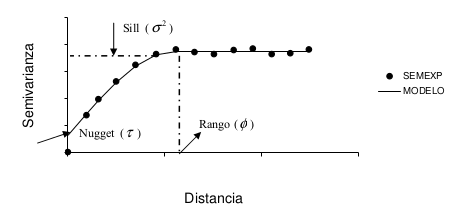
\includegraphics[scale=0.5]{teoria/images/modelo_semivarianza.png}
    \caption{SEMEXP: Semivariograma experimental y MODELO: ajuste de un modelo teórico}
    \label{modelo_semivarianza}
\end{figure}

\begin{itemize}
    \item Nugget($\tau$): Representa una discontinuidad puntual del semivariograma en el origen. Puede ser debido a errores de medición en la variable o a la escala de la misma- En algunas ocasiones puede ser indicativo de que parte de la estructura espacial se concentra a distancias inferiores a las observadas.
    \item Sill($\sigma^2$): Es un estimador de la varianza de las variables del proceso. También puede definirse como el limite del semivariograma cuando la distancia $h$ tiende a infinito
    \item Rango($\phi$) Es términos prácticos corresponde a la distancia a partir de la cual dos observaciones son independientes. El rango se interpreta como la zona de influencia. Existen algunos modelos de semivariograma en los que no existe una distancia finita para la cual dos pbservaciones sean independientes; por ello se llama rango efectivo a la distancia para la cual el semivariograma alcanza el $95\%$ de la meseta (sill) 
\end{itemize}

 Algunos de modelos más comunes y que son presentados por (Armstrong, 1950 )\cite{armstrong} son los siguientes

\subparagraph{Efecto Pepita}

Corresponde a un modelo puramente aleatorio (ruido blanco), donde no existe correlación entre los
valores sin importar la cercanía entre los mismos.

\begin{equation*}
\gamma(h) = 
\left\{ 
\begin{aligned}
0  ,&   h =0\\
C ,& |h| > 0
\end{aligned}
\right.
\end{equation*}

\subparagraph{Modelo esférico}

Es el modelo más utilizado, se compone de una expresión polinómica simple y su forma coincide con
lo observado generalmente; inicialmente un crecimiento casi lineal hasta cierta distancia y luego la
estabilización, alcanzada en un punto cuya abscisa sea $2a\sqrt{3}$

\begin{equation*}
\gamma(h) = 
\left\{ 
\begin{aligned}
C\left( \frac{3|h|}{2a} - \frac{|h|^3}{2a^3}\right) & ,   & |h| > 0\\
C & ,   & |h| > 0
\end{aligned}
\right.
\end{equation*}


\subparagraph{Modelo exponencial}
El rango efectivo de este modelo se encuentra en $a$, al ser la distancia en la cual se alcanza el $95\%$ de su límite; este modelo tiene un comportamiento lineal para distancias pequeñas, en el caso del exponencial inicialmente presenta un crecimiento muy rápido.

\begin{equation*}
\gamma(h) = 
\{C (1- exp(-|h|/a))\}
\end{equation*}

\subparagraph{Modelo Gaussiano}
Representa un fenómeno extremadamente continuo, donde se ha evidenciando la ocurrencia de
inestabilidades numéricas cuando no se hace uso del efecto pepita. Su rango efectivo es $\sqrt{3}a$.


\begin{equation*}
\gamma(h) = 
\{C (1- exp(-|h|^2/a^2))\}
\end{equation*}







\subsubsection{Métodos de Interpolación}

Una vez realizado el modelamiento del semivariograma, la predicción en puntos no muéstrales se puede hacer aplicando la técnica de interpolación Kriging. proceso que calcula el promedio ponderado de las observaciones muestrales.

 En el siguiente cuadro se mencionan los tipos de kriging

\begin{tabular}{cc}
\hline
Métodos Geoestadísticos& Nombre  \\ \hline
LINEAL & Kriging Simple \\
&Kriging Ordinario \\
& Kriging Universal \\ \hline
NO LINEAL & Kriging Indicador  \\
&Kriging Probabilístico  \\
\hline
Métodos Determinísticos& Nombre\\\hline
&IDW\\
&Interpolación polinomial local \\
&Interpolación polinomial global\\
&Funciones de base radial \\
&Polígonos de Voronoi \\
\hline


\end{tabular}




%\subsection{Propiedades}

%Es insesgado $E(Z)= \mu$, es $\mu$ porque media es constalte

\subsubsection{Selección de interpolación}
La selección del
método por medio de una validación cruzada. Con los métodos Kriging cuando se hace un pronóstico se obtiene como resultado el mismo
valor que se observó por lo que en principio la evaluación de los errores al realizar
pronósticos se dificulta.
La validación cruzada consiste en quitar un punto considerado en el modelamiento del
semivariograma para realizar los pronósticos apoyados en los métodos de interpolación,
con esto se genera un error que se asocia al coeficiente de determinación, $R^2$ , en
econometría. 

\subsubsection{Mapas y Análisis}

Una vez se ha evaluado el buen ajuste del modelo de semivarianza a los datos y se ha
verificado la bondad de los datos obtenidos con los métodos de interpolación, se elaboran salidas como los mapas de probabilidad y de desviaciones estándar, acompañados de su interpretación y análisis.




